\lab{Applications}{Earthquakes}{Earthquakes}
\objective{Cluster the epicenters of earthquakes via the k-means algorithm}

Suppose we are interested in learning about which regions are prone to experience frequent earthquake activity. We could make a map of all earthquakes over a given period of time and examine it ourselves, but we recognize this as an unsupervised learning problem and are eager to apply our new k-means clustering tool.

We have 6 .txt files, each containing a months worth of earthquake data throughout the world, from January 2010 through June 2010. These files contain a lot of information which we aren't interested in at the time; all we would like to extract from them is the location of each earthquake, which appears in characters $21$ through $33$ of each line. Characters $21$ through $26$ contain the latitude of each epicenter, character $26$ denoting North or South, and characters $27$ through $33$ contain the longitude of each epicenter, character $33$ denoting East or West. We need to divide each value by $1,000$ to represent these as degrees and decimals.

We might think that we can regard any epicenter as a point in $\mathbb{R}^{2}$ with coordinates being their latitude and longitude. This, however, would be incorrect, because the earth is not flat. We must recognize that latitude and longitude are best viewed as a variation of spherical coordinates in $\mathbb{R}^{3}$, and we should interpret them as such. Each point in $\mathbf{R}^{3}$ can be represented in Euclidean coordinates as a triple $(x,y,z)$, or in spherical coordinates as a triple $(r,\theta,\phi)$, where $r$ is the distance from the origin, $\theta$ is the angle made with the $z$-axis, and $\phi$ is the angle made by the projection onto the $x-y$ plane and the $x$-axis. Because we are considering a sphere (the earth), we can assume its radius is $1$, and ignore it throughout.

\begin{problem}
Write a function which accepts a file name of earthquake data and extracts the latitude and longitude of each earthquake epicenter. Transform these coordinates into spherical coordinates. To do this, we have to recognize that in spherical coordinates, the polar angle is measured from the north pole, not from the equator, being a transformation of the latitudes. See the figures below. The longitudes should not require a transformation. Write another function that does this for all files in the directory containing the earthquake data and returns all epicenters in spherical coordinates, with $r = 1$.
\end{problem}

\begin{figure}[h]
\centering
	\begin{tabular}{cc}
		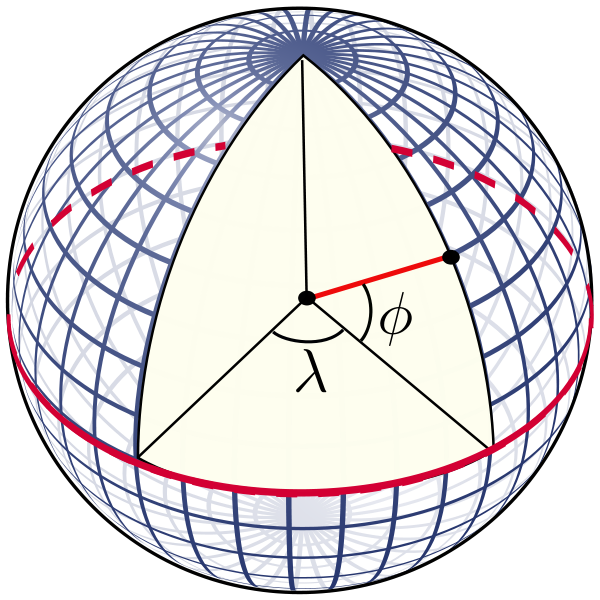
\includegraphics[width=.49\textwidth]{latlong.png}
		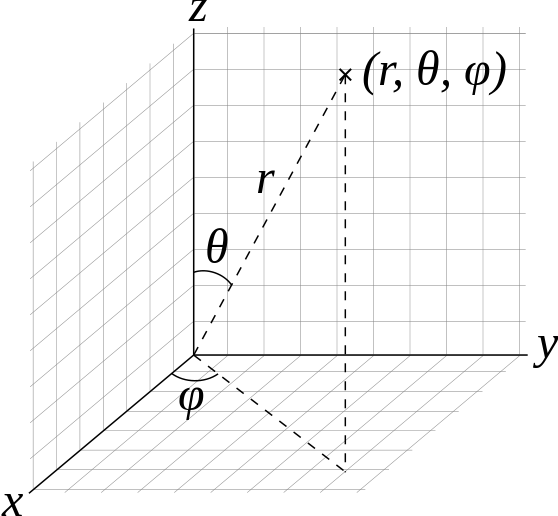
\includegraphics[width=.49\textwidth]{spherical.png}
	\end{tabular}
	\caption{Longitude and Latitude vs. Spherical Coordinates}
\end{figure}

Recall the transformations from spherical coordinates to Euclidean coordinates, and vice-versa:
\begin{align*}
r & = \sqrt{x^{2} + y^{2} + z^{2}} & x & = r \sin \theta \cos \phi \\
\theta & = \arccos \frac{z}{r} & y & = r \sin \theta \sin \phi \\
\phi & = \arctan \frac{y}{x} & z & = r \cos \theta
\end{align*}

\begin{problem}
Write three functions, one that transforms data from spherical coordinates to Euclidean coordinates, another that reverses this transformation, and a third which transforms data from spherical coordinates to latitude and longitude.
\end{problem}

\begin{problem}
Load all of the earthquake epicenters data and transform them into Euclidean coordinates in $\mathbb{R}^{3}$. Cluster the earthquakes into $15$ clusters, being sure to normalize your centroids at each step (thus keeping the earthquakes on the surface of the earth).
\end{problem}

\begin{problem}
Transform your epicenters data and your final centroids into latitude and longitude pairs and plot each cluster with a different color, as well as each centroid with a ``+'' symbol as before. You should be able to recognize geographical features (North America, the Asian Pacific coast, etc.), and see different regions of earthquake activity as in Figure \ref{fig:earthquakeclusters}. If not, then you did something wrong. What weaknesses of k-means can you see from this application problem?
\end{problem}
\begin{figure} 
	\centering
	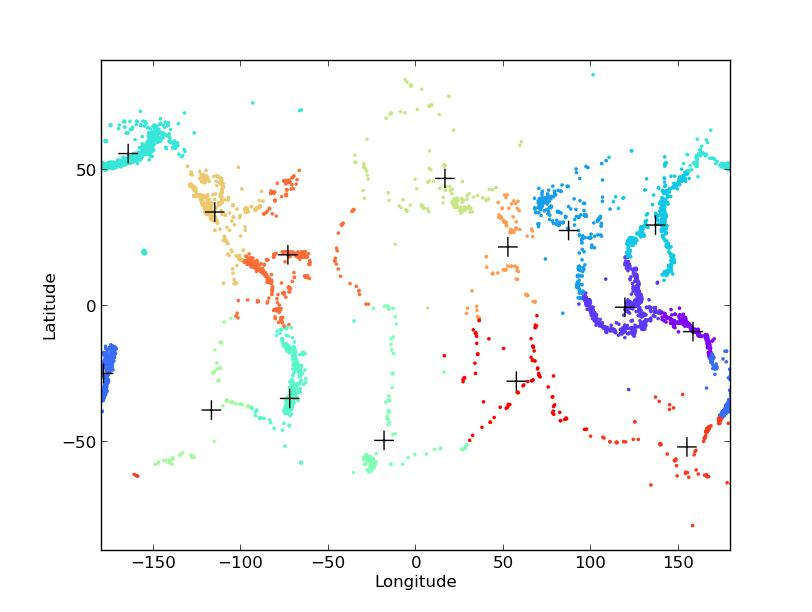
\includegraphics[width=\textwidth]{clusters.jpg}
	\caption{Earthquake epicenter clusters with $N = 15$}
	\label{fig:earthquakeclusters}
\end{figure}